\documentclass[12pt]{article}
\usepackage[brazil]{babel}
\usepackage[utf8]{inputenc}
\usepackage[T1]{fontenc}
\usepackage{amsmath, amssymb}
\usepackage{geometry}
\usepackage{graphicx}
\usepackage{tikz}
\usetikzlibrary{shapes.gates.logic.US, positioning, calc}
\usepackage{xcolor}
\usepackage{enumitem}
\usepackage{fancyhdr}
\usepackage[most]{tcolorbox}

% Definição de Cores (Padrão UniRV)
\definecolor{forestgreen}{RGB}{0,100,50}
\definecolor{maincolor}{RGB}{0,100,50}

% Configuração de Box
\newtcolorbox{block}[1]{%
  colback=green!5,
  colframe=maincolor,
  coltitle=white, 
  title=#1,
  fonttitle=\bfseries,
  boxrule=1.5pt,
  arc=3mm,
  left=6pt,
  right=6pt,
  top=6pt,
  bottom=6pt
}

% Geometria e Header
\geometry{margin=2.5cm, headheight=53pt, top=2.5cm}
\pagestyle{fancy}
\fancyhf{}

\renewcommand{\headrulewidth}{2pt}
\renewcommand{\footrulewidth}{2pt}

\renewcommand{\headrule}{\hbox to\headwidth{%
  \color{forestgreen}\leaders\hrule height \headrulewidth\hfill}}

\renewcommand{\footrule}{\hbox to\headwidth{%
  \color{forestgreen}\leaders\hrule height \footrulewidth\hfill}}

\fancyhead[L]{%
  
\includegraphics[height=1.2cm]{Universidade_de_Rio_Verde.jpg}
}

\fancyhead[R]{%
  \raggedleft
  \textcolor{forestgreen}{%
    \footnotesize 
    \textbf{Exercício — Display de 7 Segmentos}
    Me.~Sergio Souza Novak\\
    \textit{Lógica para Engenharia de Software}
  }
}

\fancyfoot[C]{%
  \textcolor{forestgreen}{\thepage}
}

\begin{document}

\section*{O que é um Display de 7 Segmentos?}

O display de 7 segmentos é um componente eletrônico utilizado para exibir dígitos decimais e alguns caracteres alfanuméricos. Ele consiste em sete LEDs (segmentos) organizados em um padrão de "8". Ao acender diferentes combinações desses LEDs, podemos representar os números de 0 a 9.

\begin{itemize}
    \item \textbf{Catodo Comum:} Todos os catodos dos LEDs estão conectados ao terra. Os segmentos acendem com nível lógico \textbf{HIGH (1)}.
    \item \textbf{Anodo Comum:} Todos os anodos dos LEDs estão conectados ao VCC. Os segmentos acendem com nível lógico \textbf{LOW (0)}.
\end{itemize}

Neste exercício, assumiremos um display de \textbf{Catodo Comum}, onde os segmentos acendem em nível lógico \textbf{1}.

\subsection*{Diagrama do Display}

Abaixo está a representação dos segmentos, identificados pelas letras de \textbf{a} a \textbf{g}.

\begin{center}
    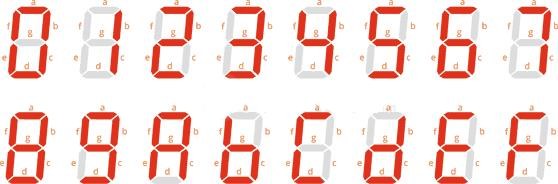
\includegraphics[height=4.2cm]{7segmentos.jpg}
    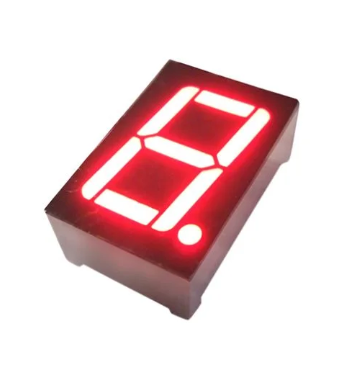
\includegraphics[height=4.2cm]{display.png}

\end{center}

\vspace{0.5cm}

\section*{Tabela de Decodificação (0--9)}

Para controlar o display, utilizamos 4 entradas binárias ($A, B, C, D$) que representam o valor em binário (BCD) e 7 saídas ($a, b, c, d, e, f, g$), uma para cada segmento.

\begin{block}{Entradas e Saídas}
  \textbf{Entradas}: $A$ (MSB), $B, C, D$ (LSB) \\
  \textbf{Saídas}: $a, b, c, d, e, f, g$ (Nível 1 acende)
\end{block}

\begin{center}
\renewcommand{\arraystretch}{1.3}
\begin{tabular}{|c|c|cccc|ccccccc|}
\hline
\textbf{Decimal} & \textbf{Hexa} & \textbf{A} & \textbf{B} & \textbf{C} & \textbf{D} & \textbf{a} & \textbf{b} & \textbf{c} & \textbf{d} & \textbf{e} & \textbf{f} & \textbf{g} \\ \hline
0 & 0 & 0 & 0 & 0 & 0 & 1 & 1 & 1 & 1 & 1 & 1 & 0 \\ \hline
1 & 1 & 0 & 0 & 0 & 1 & 0 & 1 & 1 & 0 & 0 & 0 & 0 \\ \hline
2 & 2 & 0 & 0 & 1 & 0 & 1 & 1 & 0 & 1 & 1 & 0 & 1 \\ \hline
3 & 3 & 0 & 0 & 1 & 1 & 1 & 1 & 1 & 1 & 0 & 0 & 1 \\ \hline
4 & 4 & 0 & 1 & 0 & 0 & 0 & 1 & 1 & 0 & 0 & 1 & 1 \\ \hline
5 & 5 & 0 & 1 & 0 & 1 & 1 & 0 & 1 & 1 & 0 & 1 & 1 \\ \hline
6 & 6 & 0 & 1 & 1 & 0 & 1 & 0 & 1 & 1 & 1 & 1 & 1 \\ \hline
7 & 7 & 0 & 1 & 1 & 1 & 1 & 1 & 1 & 0 & 0 & 0 & 0 \\ \hline
8 & 8 & 1 & 0 & 0 & 0 & 1 & 1 & 1 & 1 & 1 & 1 & 1 \\ \hline
9 & 9 & 1 & 0 & 0 & 1 & 1 & 1 & 1 & 1 & 0 & 1 & 1 \\ \hline
\end{tabular}
\end{center}

\vspace{0.5cm}

\section*{Exercício}

Utilizando a tabela acima, encontre as expressões booleanas simplificadas (Álgebra de Boole) para cada um dos segmentos. Considere apenas os dígitos de 0 a 9 (entradas 0000 a 1001).

\newpage

\section*{Resolução Detalhada (Simplificação por Literais)}

Abaixo, apresentamos a manipulação algébrica completa para cada LED, utilizando os literais e as propriedades da Álgebra Booleana.

\subsection*{LED \textbf{a}}
\textbf{Forma Canônica:}
\[ a = \bar{A}\bar{B}\bar{C}\bar{D} + \bar{A}\bar{B}C\bar{D} + \bar{A}\bar{B}CD + \bar{A}B\bar{C}D + \bar{A}BC\bar{D} + \bar{A}BCD + A\bar{B}\bar{C}\bar{D} + A\bar{B}\bar{C}D \]

\textbf{Simplificação (Conta Toda):}
\begin{enumerate}
    \item Agrupando termos com $\bar{A}C$:
    $(\bar{A}\bar{B}C\bar{D} + \bar{A}\bar{B}CD + \bar{A}BC\bar{D} + \bar{A}BCD) = \bar{A}C(\bar{B}\bar{D} + \bar{B}D + B\bar{D} + BD) = \bar{A}C(1) = \bar{A}C$
    \item Agrupando termos com $\bar{A}BD$:
    $(\bar{A}B\bar{C}D + \bar{A}BCD) = \bar{A}BD(\bar{C} + C) = \bar{A}BD(1) = \bar{A}BD$
    \item Agrupando termos com $\bar{B}\bar{C}\bar{D}$:
    $(\bar{A}\bar{B}\bar{C}\bar{D} + A\bar{B}\bar{C}\bar{D}) = \bar{B}\bar{C}\bar{D}(\bar{A}+A) = \bar{B}\bar{C}\bar{D}(1) = \bar{B}\bar{C}\bar{D}$
    \item Agrupando termos com $A\bar{B}\bar{C}$:
    $(A\bar{B}\bar{C}\bar{D} + A\bar{B}\bar{C}D) = A\bar{B}\bar{C}(\bar{D}+D) = A\bar{B}\bar{C}(1) = A\bar{B}\bar{C}$
\end{enumerate}

\begin{block}{Resultado Final do LED a}
  \[ a = \bar{A}C + \bar{A}BD + \bar{B}\bar{C}\bar{D} + A\bar{B}\bar{C} \]
\end{block}

\subsection*{LED \textbf{b}}
\textbf{Forma Canônica:}
\[ b = \bar{A}\bar{B}\bar{C}\bar{D} + \bar{A}\bar{B}\bar{C}D + \bar{A}\bar{B}C\bar{D} + \bar{A}\bar{B}CD + \bar{A}B\bar{C}\bar{D} + \bar{A}BCD + A\bar{B}\bar{C}\bar{D} + A\bar{B}\bar{C}D \]

\textbf{Simplificação (Conta Toda):}
\begin{enumerate}
    \item $(\bar{A}\bar{B}\bar{C}\bar{D} + \bar{A}\bar{B}\bar{C}D + \bar{A}\bar{B}C\bar{D} + \bar{A}\bar{B}CD) = \bar{A}\bar{B}(\text{Complemento}) = \bar{A}\bar{B}$
    \item $(\bar{A}\bar{B}\bar{C}\bar{D} + \bar{A}B\bar{C}\bar{D}) = \bar{A}\bar{C}\bar{D}(\bar{B}+B) = \bar{A}\bar{C}\bar{D}$
    \item $(\bar{A}\bar{B}\bar{C}\bar{D} + A\bar{B}\bar{C}\bar{D}) = \bar{B}\bar{C}\bar{D}(\bar{A}+A) = \bar{B}\bar{C}\bar{D}$
    \item $(\bar{A}\bar{B}CD + \bar{A}BCD) = \bar{A}CD(\bar{B}+B) = \bar{A}CD$
    \item $(A\bar{B}\bar{C}\bar{D} + A\bar{B}\bar{C}D) = A\bar{B}\bar{C}(\bar{D}+D) = A\bar{B}\bar{C}$
\end{enumerate}
\begin{block}{Resultado Final do LED b}
  \[ b = \bar{A}\bar{B} + \bar{A}\bar{C}\bar{D} + \bar{B}\bar{C}\bar{D} + \bar{A}CD + A\bar{B}\bar{C} \]
\end{block}

\subsection*{LED \textbf{c}}
\textbf{Forma Canônica:} $m_0, m_1, m_3, m_4, m_5, m_6, m_7, m_8, m_9$
\begin{enumerate}
    \item $(\bar{A}B\bar{C}\bar{D} + \bar{A}B\bar{C}D + \bar{A}BC\bar{D} + \bar{A}BCD) = \bar{A}B$
    \item $(\bar{A}\bar{B}\bar{C}D + \bar{A}\bar{B}CD + \bar{A}B\bar{C}D + \bar{A}BCD) = \bar{A}D$
    \item $(\bar{A}\bar{B}\bar{C}\bar{D} + \bar{A}\bar{B}\bar{C}D + A\bar{B}\bar{C}\bar{D} + A\bar{B}\bar{C}D) = \bar{B}\bar{C}$
    \item $(A\bar{B}\bar{C}\bar{D} + A\bar{B}\bar{C}D) = A\bar{B}\bar{C}$
\end{enumerate}
\begin{block}{Resultado Final do LED c}
  \[ c = \bar{A}B + \bar{A}D + \bar{B}\bar{C} + A\bar{B}\bar{C} \]
\end{block}

\newpage

\subsection*{LED \textbf{d}}
\textbf{Forma Canônica:} $m_0, m_2, m_3, m_5, m_6, m_8, m_9$
\begin{enumerate}
    \item $(\bar{A}\bar{B}C\bar{D} + \bar{A}\bar{B}CD) = \bar{A}\bar{B}C$
    \item $(\bar{A}\bar{B}C\bar{D} + \bar{A}BC\bar{D}) = \bar{A}C\bar{D}$
    \item Termo isolado: $\bar{A}B\bar{C}D$
    \item $(\bar{A}\bar{B}\bar{C}\bar{D} + A\bar{B}\bar{C}\bar{D}) = \bar{B}\bar{C}\bar{D}$
    \item $(A\bar{B}\bar{C}\bar{D} + A\bar{B}\bar{C}D) = A\bar{B}\bar{C}$
\end{enumerate}
\begin{block}{Resultado Final do LED d}
  \[ d = \bar{A}\bar{B}C + \bar{A}C\bar{D} + \bar{A}B\bar{C}D + \bar{B}\bar{C}\bar{D} + A\bar{B}\bar{C} \]
\end{block}

\subsection*{LED \textbf{e}}
\textbf{Forma Canônica:} $\bar{A}\bar{B}\bar{C}\bar{D} + \bar{A}\bar{B}C\bar{D} + \bar{A}BC\bar{D} + A\bar{B}\bar{C}\bar{D}$
\begin{enumerate}
    \item $(\bar{A}\bar{B}\bar{C}\bar{D} + A\bar{B}\bar{C}\bar{D}) = \bar{B}\bar{C}\bar{D}(\bar{A}+A) = \bar{B}\bar{C}\bar{D}$
    \item $(\bar{A}\bar{B}C\bar{D} + \bar{A}BC\bar{D}) = \bar{A}C\bar{D}(\bar{B}+B) = \bar{A}C\bar{D}$
\end{enumerate}
\begin{block}{Resultado Final do LED e}
  \[ e = \bar{B}\bar{C}\bar{D} + \bar{A}C\bar{D} \]
\end{block}

\subsection*{LED \textbf{f}}
\textbf{Forma Canônica:} $m_0, m_4, m_5, m_6, m_8, m_9$
\begin{enumerate}
    \item $(\bar{A}B\bar{C}\bar{D} + \bar{A}B\bar{C}D) = \bar{A}B\bar{C}$
    \item $(\bar{A}B\bar{C}\bar{D} + \bar{A}BC\bar{D}) = \bar{A}B\bar{D}$
    \item $(\bar{A}\bar{B}\bar{C}\bar{D} + A\bar{B}\bar{C}\bar{D}) = \bar{B}\bar{C}\bar{D}$
    \item $(A\bar{B}\bar{C}\bar{D} + A\bar{B}\bar{C}D) = A\bar{B}\bar{C}$
\end{enumerate}
\begin{block}{Resultado Final do LED f}
  \[ f = \bar{A}B\bar{C} + \bar{A}B\bar{D} + \bar{B}\bar{C}\bar{D} + A\bar{B}\bar{C} \]
\end{block}

\subsection*{LED \textbf{g}}
\textbf{Forma Canônica:} $m_2, m_3, m_4, m_5, m_6, m_8, m_9$
\begin{enumerate}
    \item $(\bar{A}\bar{B}C\bar{D} + \bar{A}\bar{B}CD) = \bar{A}\bar{B}C$
    \item $(\bar{A}\bar{B}C\bar{D} + \bar{A}BC\bar{D}) = \bar{A}C\bar{D}$
    \item $(\bar{A}B\bar{C}\bar{D} + \bar{A}B\bar{C}D) = \bar{A}B\bar{C}$
    \item $(A\bar{B}\bar{C}\bar{D} + A\bar{B}\bar{C}D) = A\bar{B}\bar{C}$
\end{enumerate}
\begin{block}{Resultado Final do LED g}
  \[ g = \bar{A}\bar{B}C + \bar{A}C\bar{D} + \bar{A}B\bar{C} + A\bar{B}\bar{C} \]
\end{block}

\end{document}
